%% Auto-generated from paper_template.tex by 10_build_paper.py; every number is read from discovery_results.json.
\documentclass[aps,prd,twocolumn,superscriptaddress,nofootinbib,floatfix,10pt]{revtex4-2}
\usepackage{amsmath,amssymb,graphicx,booktabs,array}
\usepackage[colorlinks=true,allcolors=blue]{hyperref}
\newcommand{\eps}{\varepsilon}
\newcommand{\lC}{\lambda_C}
\newcommand{\MPl}{M_{\rm Pl}}
\begin{document}

\title{Beyond the static Einstein--Euler--Heisenberg description of an extreme electric field:\\ a formally verified validity map for discharge and trapping}

\author{\'Alvaro L\'opez Almeida}
\date{\today}

\begin{abstract}
We ask what lies beyond the point where the static, quartic-truncated Einstein--Euler--Heisenberg (EEH) description of a point-like electric charge breaks down ($\eps\equiv eE/m_e^2\gtrsim 1$, $r\lesssim\lC$), and whether QED can act as a ``universal quantum censor'' that prevents the gravitational collapse of the field. Every equation used is derived or checked with a computer algebra system (123 gates, 25 of them negative controls that must fail on altered models). We find: (i) the exact one-loop (proper-time) real part does not saturate the field; it reproduces Reissner--Nordstr\"om with a running charge, whereas the quartic truncation and a matched Born--Infeld model yield a spurious single Schwarzschild-like horizon; the dominant-energy condition is violated for $\eps>$1.88218 with relative margin $\to-\alpha/3\pi$ (the one-loop trace anomaly). (ii) The condition $\theta_+=0\Leftrightarrow 2GM_{\rm MS}=R$, the decomposition $M_{\rm ADM}=M_{\rm MS}(R)+U_C(R)$ and the exact cancellation of the electrostatic energy are derived inside the pipeline for time-symmetric spherical data, together with the exact one-loop correction to $U_C$. (iii) A Pauli-blocked Markov kinetic model keeps $0\le f\le \tfrac12$ and gives $\omega_p=$0.186$\,e\sqrt{eE_0}$; replacing the Markov ansatz by the exact Bloch--Bogoliubov equations coupled to Maxwell's equation (the normalization of the coupling is fixed by a Landau--Zener test) lets the occupation reach $f_{\max}=$1.0000, advances the first field zero by 19 per cent, raises the plasma frequency to $\omega_p=$0.194$\,e\sqrt{eE_0}$, and shows that the pairs form a collinear gas with $\langle w_\parallel\rangle=$0.99 rather than $\tfrac13$, with energy conserved to \ensuremath{6.2\times10^{-12}}. (iv) The ratio of the discharge time to the free-fall time obeys $\tau_{\rm dis}/\tau_{\rm ff}=(r_0^*/r_0)^{1/2}$ with $r_0^*$ independent of the number of charges $N$, and a quantitative $(N,r_0)$ phase map is given.  (v) Without time symmetry, the Misner--Sharp balance $\partial_tM_{\rm MS}=-4\pi r^2F_{\rm flux}$ is derived and the internal field-to-plasma conversion is shown to leave $M_{\rm MS}$ unchanged; a 1+1D solver of the discharge of a charged ball in general relativity shows that the plasma leaving through the surface removes only a fraction 0.50 of the interior field energy while the ingoing half of the plasma converted outside adds $2.5$ times more, so the net effect is a gain; the dynamics shifts the critical mass by less than 0.8 per cent, and the horizon boundary is set instead by the static interior field energy, which places the shell curve $r_s(N)$ inside an initial apparent horizon for $N>$\ensuremath{4.6\times10^{4}}. (vi) The matter is evolved as a charged thin shell inside the general-relativistic solver, fully coupled to the plasma and the field (the energy of the whole system is conserved to \ensuremath{5\times10^{-4}}): without discharge it collapses only if $q<C/2$; with discharge, the gravity of the plasma generated by the field itself binds it, lowering the screening speed needed to avoid the Coulomb explosion by a factor 0.24 at $(q,C)=(1,0.1)$ relative to the decoupled law $s_c=0.66\,q^2/C^{3/2}$ (verified by simulation to \ensuremath{1.8\times10^{-2}}); the mass at the shell does not decrease but rises, by Coulomb work and by plasma inflow. Several ingredients are known results that we re-derive and verify; Sec.~\ref{sec:attrib} separates them from what is specific to this work, and Sec.~\ref{sec:limits} states the regimes where the model is not controlled.
\end{abstract}

\maketitle

\section{Introduction}\label{sec:intro}
The Euler--Heisenberg (EH) effective action \cite{heisenberg1936,weisskopf1936,schwinger1951} coupled to Einstein gravity has been used to study QED corrections to charged black holes in its quartic truncation \cite{yajima2001,ruffini2013}. Its validity requires $\eps\ll1$, and for a point charge $Q=Ne$ the static field reaches $\eps=1$ at $r_\eps=\sqrt{N\alpha}\,\lC$, long before any horizon unless $N\gtrsim N_{\rm crit}=\MPl^2/m_e^2\simeq$\ensuremath{5.71\times10^{44}}. Beyond that point two qualitatively different effects matter: nonperturbative vacuum pair creation, which discharges the field on plasma time scales \cite{kluger1991,kluger1992,kluger1998,ruffini2010,gelis2016}, and the gravitational response, which depends on whether a trapped surface can exist at all. The loss of charge by black holes through a Schwinger-type mechanism goes back to Gibbons \cite{gibbons1975}, and the structure of charged thin-shell collapse to Israel, Boulware and Bekenstein \cite{boulware1973,bekenstein1971}.

\textbf{Aim and scope.} We do not claim a new law of nature. We build a reproducible, formally gated computation that (a) quantifies where the quartic EEH extrapolation is qualitatively wrong, (b) re-derives the trapping criterion without invoking external theorems, (c) extends the pair-plasma back-reaction through several field reversals with Pauli blocking, and (d) assembles the resulting scales in one phase map. The pipeline (Appendix~\ref{app:pipeline}) executes symbolic derivations (SymPy), adaptive numerical integrations with independent cross-checks, and negative controls; it fails if any gate fails. All numbers quoted below are read automatically from the pipeline output.

\section{Static nonlinear electrodynamics coupled to gravity}\label{sec:static}
\subsection{Reduction for an arbitrary $\mathcal L(E)$}
For the static spherical ansatz $ds^2=-f\,dt^2+dr^2/g+r^2d\Omega^2$, $A=\Phi(r)\,dt$, a purely electric field $E=\sqrt{g/f}\,\Phi'$ and any Lagrangian $\mathcal L(X)$, $X=F_{\mu\nu}F^{\mu\nu}=-2E^2$, the stress tensor derived from the full tensor expression obeys
\begin{align}
T^t{}_t&=T^r{}_r=-\rho,\quad \rho=E\mathcal L'-\mathcal L,\quad T^\theta{}_\theta=\mathcal L,\label{eq:T}\\
r^2\mathcal L'(E)&=Q/4\pi,\qquad f=g=1-\frac{2Gm(r)}{r},\quad m'=4\pi r^2\rho,\label{eq:red}
\end{align}
and $\rho'=-(2/r)(\rho+p_\perp)$ holds identically (gates S1--S4; the control C1 with $p_\perp=\mathcal L/2$ is detected). For Maxwell, $\rho=E^2/2$; for the quartic EH term, $\mathcal L=E^2/2+4cE^4$ with $c=\alpha^2/90\,m_e^4$.

\subsection{One-loop proper-time Lagrangian and strong-field behaviour}
For purely electric fields the spinor one-loop correction is
\begin{equation}
\mathcal L_1(x)=-\frac{1}{8\pi^2}\!\int_0^\infty\!\frac{ds}{s^3}e^{-s}\Big[xs\cot(xs)-1+\tfrac{(xs)^2}{3}\Big],\ \ x=e E,
\end{equation}
evaluated on the ray $s=\rho e^{-i\pi/4}$ because the poles of $\cot$ lie on the real axis. The real part is the effective Lagrangian; the imaginary part reproduces the Schwinger series $\mathrm{Im}\,\mathcal L_1=\frac{x^2}{8\pi^3}\sum_n n^{-2}e^{-n\pi/x}$ to a relative error of \ensuremath{8.5\times10^{-15}} (gate N1), and for $\eps\ll1$ it matches $4cE^4$ with $\mathcal L_1/(4cE^4)-1\propto\eps^{2.00}$ (N2; the Taylor coefficient is checked symbolically, S6).

At strong field the expansion is logarithmic, in agreement with the known renormalization-group structure \cite{ritus1975,dunne2004}:
\begin{equation}
\mathcal L=\frac{E^2}{2}\Big[1-\frac{\alpha}{3\pi}\big(\ln\eps+3K\big)\Big],\quad K=\ensuremath{-0.7640},
\label{eq:log}
\end{equation}
where the coefficient is verified symbolically (S7) and the slope $d(\mathcal L_1/x^2)/d\ln x=\ensuremath{-4.22171597\times10^{-3}}$ agrees with $-1/24\pi^2=\ensuremath{-4.22171599\times10^{-3}}$ (N3). The pole of Eq.~(\ref{eq:log}) sits at $\log_{10}\eps_L=561.9$, i.e.\ $\mu_L=\sqrt{eE}\approx10^{277.7}$~GeV, consistent with the usual Landau scale of QED, whereas the Planck density corresponds to $\log_{10}\eps_{\rm Pl}=44.4$. This holds \emph{at one loop}: the Ritus--Narozhny conjecture, that each loop in a strong field costs $\alpha\chi^{2/3}$ and perturbation theory fails for $\chi\gtrsim\alpha^{-3/2}\simeq1604$ \cite{fedotov2017,fedotov2023}, would invalidate all one-loop statements far below $\eps_L$; its applicability to a pure electric field is not established here.

\subsection{Energy conditions and the trace anomaly}
WEC and NEC hold for the one-loop Lagrangian up to $\eps=10^{40}$ (the minima of $\rho/E^2$ and $ED/E^2$ are 0.465 and 0.930, gate N7), and $\mathcal L>0$ (SEC) until the pole (N8). The dominant energy condition $\rho\ge|p_\perp|$ requires $ED-2\mathcal L\ge0$, and SymPy establishes the identity (gate S10)
\begin{equation}
ED-2\mathcal L=x\mathcal L_1'-2\mathcal L_1=x^3\frac{d}{dx}\Big(\frac{\mathcal L_1}{x^2}\Big).
\end{equation}
Hence the DEC is violated exactly where $\mathcal L_1/x^2$ decreases, i.e.\ for $\eps>$1.88218 (root found with the exact integral, not the interpolation). The relative margin $(\rho-|\mathcal L|)/\rho$ tends to $-\alpha/3\pi=\ensuremath{-7.743\times10^{-4}}$ and keeps growing slowly with $\ln\eps$ (\ensuremath{-7.875\times10^{-4}} at $\eps=10^{10}$) up to the pole: it is \emph{not} bounded. This is the one-loop trace anomaly $T^\mu{}_\mu\propto\beta F^2$ \cite{adler1977,collins1977} written in terms of $\rho$ and $p_\perp$, not a new quantum violation. For nonlinear electrodynamics of Pleba\'nski class, causality implies the DEC \cite{russo2024}; the corresponding causality conditions for the full $\mathcal L_1(S,P)$ have not been evaluated here, so we do not draw a conclusion on (a)causality.

\subsection{Interior profiles}
Figure~\ref{fig:profiles} compares the metric function and the field for $N=10^6$ and $M=1.5M_{\rm ext}$. The quartic extrapolation gives $E\propto r^{-2/3}$ and a finite interior mass (gate S9), and a Born--Infeld model matched to the quartic term ($b^2=1/32c$, S5; field bounded by $\eps=69.6$) yields the same single horizon at $r=2GM$, $r_h=\ensuremath{1.07263\times10^{-17}}\,\lC$. The exact one-loop result retains two horizons, $r_-=\ensuremath{1.48259\times10^{-18}}$ and $r_+=\ensuremath{9.24904\times10^{-18}}$ (Reissner--Nordstr\"om: \ensuremath{1.36569\times10^{-18}} and \ensuremath{9.36055\times10^{-18}}), consistent with an effective charge $Q^2\to\lambda Q^2$, $\lambda=E/E_{\rm Coul}(r_+)=1.0710$: the measured shift $\delta r_+/r_+=\ensuremath{-1.191\times10^{-2}}$ agrees with the running-charge prediction \ensuremath{-1.230\times10^{-2}} (N6). The static nonlinearity therefore does not censor the horizon. These profiles are \emph{formal solutions of the locally-constant-field model}: for $r\sim r_Q$ the field varies on a scale $\ell\simeq r_Q/2\sim\ensuremath{1.8\times10^{-18}}\,\lC\ll\lC$, outside the derivative expansion (Sec.~\ref{sec:limits}).

\begin{figure*}[t]
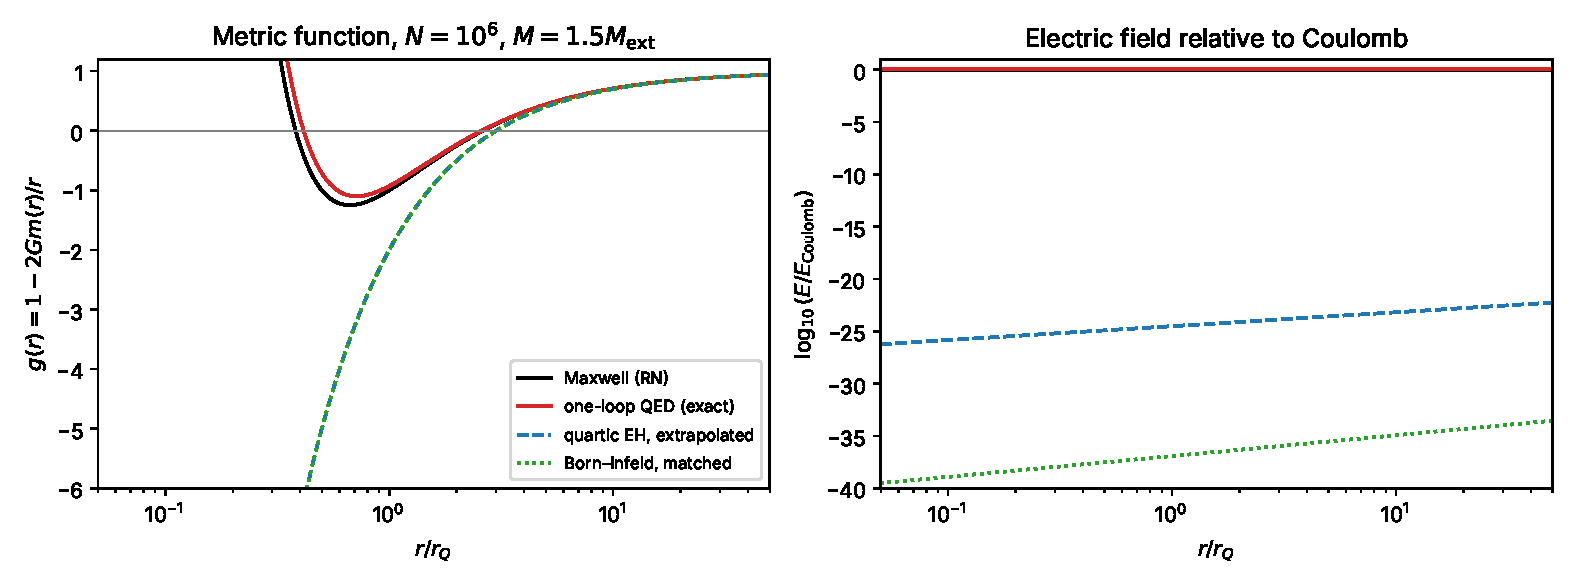
\includegraphics[width=0.92\textwidth]{fig_metric_profiles.pdf}
\caption{Metric function $g(r)=1-2Gm(r)/r$ (left) and electric field relative to Coulomb (right) for $N=10^6$ charges and $M=1.5M_{\rm ext}$, in the exact one-loop model, Maxwell (Reissner--Nordstr\"om), the quartic Euler--Heisenberg truncation extrapolated beyond its validity, and a Born--Infeld model matched to the quartic term.}
\label{fig:profiles}
\end{figure*}

\section{Trapping criterion derived inside the pipeline}\label{sec:trap}
The statement that the electrostatic energy does not help to trap a charged shell is standard in terms of the Misner--Sharp mass \cite{misner1964,hayward1994,boulware1973}; the charged Penrose inequality is a known theorem under stated hypotheses \cite{malec1994,khuri2017}. To remove any dependence on citations we derive what we use (gate \texttt{P10\_misner\_sharp\_symbolic}, 16 sub-checks).

\emph{(a) Geometry.} In double-null coordinates, $ds^2=-2e^{2\sigma}du\,dv+R^2d\Omega^2$, with $M_{\rm MS}=(R/2G)(1-g^{ab}\partial_aR\,\partial_bR)$ and expansions $\theta_\ell=2\partial_uR/R$, $\theta_n=2\partial_vR/R$, SymPy proves
\begin{equation}
1-\frac{2GM_{\rm MS}}{R}=-\frac{R^2e^{-2\sigma}}{2}\,\theta_\ell\theta_n .
\end{equation}
Hence $\theta_+=0\Leftrightarrow2GM_{\rm MS}=R$ (for $\theta_-\neq0$), and a trapped surface is $2GM_{\rm MS}>R$.

\emph{(b) Constraint.} For time-symmetric data ($K_{ij}=0$) the Hamiltonian constraint follows from computing $G_{ab}n^an^b=2Gm'/r^2$ for a metric with arbitrary second time derivatives, which drop out; thus $m'=4\pi r^2\rho$. The radial Maxwell field obeys Gauss' law $r^2E_{\rm orth}=\mathrm{const}$ independently of the metric and $T_{ab}n^an^b=E_{\rm orth}^2/2$.

\emph{(c) ADM decomposition.} Integrating from $R$ to infinity,
\begin{equation}
M_{\rm ADM}=M_{\rm MS}(R)+U_C(R),\quad U_C(R)=\frac{Q^2}{8\pi R},
\end{equation}
so the exterior metric \emph{is} Reissner--Nordstr\"om, $g=1-2GM_{\rm ADM}/r+GQ^2/4\pi r^2$ (derived, not assumed).

\emph{(d) Cancellation.} At $\theta_+=0$, $GM_{\rm ADM}=(R+r_Q^2/R)/2$ with $r_Q^2=GQ^2/4\pi$ (the equality case of the charged Penrose inequality). With $M_{\rm MS}(R)=M_n$ the electrostatic term cancels identically: $G(M_n+U_C)-\tfrac12(R+r_Q^2/R)=GM_n-R/2$. Non-charged exterior matter with $\rho\ge0$ only adds mass, giving the inequality.

\textbf{Scope.} Proven in this subsection: spherical time-symmetric data, $\rho\ge0$, no charged matter outside the surface. The dynamical case ($K_{ij}\neq0$) is treated in Sec.~\ref{sec:dyn}; the persistence of trapped surfaces under $\mathrm{NEC}$ is cited, not proven. The control C4 verifies that wrong factors in $M_{\rm MS}$, in the constraint ($m'=2\pi r^2\rho$) or in $U_C$ are detected.

\emph{One-loop correction to $U_C$.} For a general $\mathcal L$ with $H(D)=ED-\mathcal L$ and $dH/dD=E$ (proved for arbitrary $\mathcal L$), $\rho=H(D)$, $D=a/r^2$, $a=Q/4\pi$, and
\begin{equation}
U(R)=2\pi a^{3/2}\!\int_0^{D_R}\!H(D)\,D^{-5/2}dD,\quad D_R=a/R^2 ,
\end{equation}
which gives $Q^2/8\pi R$ for Maxwell and $-16\pi c\,a^4/5R^5$ for the quartic term (symbolic). With the exact one-loop $H$ and $N=10^6$, $U_{\rm QED}/U_C-1=\ensuremath{7.047\times10^{-2}}$ at $R=r_Q$, in agreement with a direct radial quadrature to \ensuremath{8.9\times10^{-14}} (gate P11). The slope with respect to $\ln\eps$ is \ensuremath{7.8527\times10^{-4}} ($\ln\eps\in[9,23]$) and \ensuremath{8.1870\times10^{-4}} ($[18,60]$), approaching $\alpha/3\pi=\ensuremath{7.7427\times10^{-4}}$ with the $O(\alpha\ln\eps)$ sub-leading logarithm.

\subsection{Dynamical Misner--Sharp balance without time symmetry}\label{sec:dyn}
For the general metric $ds^2=-e^{2\phi(t,r)}dt^2+e^{2\lambda(t,r)}dr^2+r^2d\Omega^2$ and $M_{\rm MS}=(r/2G)(1-e^{-2\lambda})$, SymPy computes the full Einstein tensor and proves $G^t{}_t=-2GM_r/r^2$ and $G^r{}_t=2GM_t/r^2$, i.e.\
\begin{equation}
\partial_rM_{\rm MS}=4\pi r^2\rho,\qquad \partial_tM_{\rm MS}=4\pi r^2T^r{}_t=-4\pi r^2F_{\rm flux},\quad F_{\rm flux}\equiv-T^r{}_t ,\label{eq:msdyn}
\end{equation}
together with $K^r{}_r=-e^{-\phi}\partial_t\lambda=-4\pi Gre^{2\lambda-\phi}T^r{}_t$ and $K^\theta{}_\theta=0$ (D\_MS1): the slices have $K_{ij}\neq0$ if and only if there is an energy flux, so the data of gate P10 are exactly the zero-flux case. For a radial electric field (the Maxwell tensor is built from $F_{tr}=-e^{\phi+\lambda}E$, with $T^t{}_t=T^r{}_r=-E^2/2$, $T^\theta{}_\theta=E^2/2$ and $T^r{}_t=0$) SymPy verifies $\nabla_\mu T^\mu{}_\nu{}^{\rm (EM)}=F_{\nu\lambda}J^\lambda$ in the dynamical metric, with $J^\nu\equiv\nabla_\mu F^{\mu\nu}$, and that its $t$-component is $-\partial_t(E^2/2)$. If the plasma obeys $\nabla_\mu T^{\mu}{}_\nu{}^{\rm (pl)}=-F_{\nu\lambda}J^\lambda$, the two Einstein constraints $G^r{}_t$ and $G^r{}_r-G^t{}_t$ give
\begin{equation}
\partial_t\rho_{\rm tot}=\frac1{r^2}\partial_r\!\big(r^2T^r{}_t\big)\quad\text{independently of }F_{t\lambda}J^\lambda ,
\end{equation}
so the internal conversion $E^2/2\to\rho_{\rm pl}$ in $r<R$ conserves $M_{\rm MS}(t,R)$ exactly and $\partial_tM_{\rm MS}(t,R)=4\pi R^2T^r{}_t(R)$ depends only on the plasma flux through $r=R$ (D\_MS2); if the transfer law is altered to $(1+\delta)F_{t\lambda}J^\lambda$ a spurious volume source $4\pi\delta\!\int_0^Rr^2F_{t\lambda}J^\lambda dr$ appears (control C\_MS). For a boundary $r=R(t)$, $dM_{\rm MS}/dt=4\pi R^2(T^r{}_t+\dot R\rho)$ vanishes for comoving matter, so only the flux \emph{relative} to the surface matters (D\_MS3). Radial null streams $T^{\mu\nu}=\rho_\pm\ell_\pm^\mu\ell_\pm^\nu$ propagate with $v=\alpha/a=e^{\phi-\lambda}$ and, with $W_\pm=r^2\rho_\pm$,
\begin{align}
\partial_tW_++\partial_r(vW_+)&=-W_+\big[v(\phi_r+\lambda_r)+2\lambda_t\big],\label{eq:null1}\\
\partial_tW_--\partial_r(vW_-)&=+W_-\big[v(\phi_r+\lambda_r)-2\lambda_t\big],\label{eq:null2}
\end{align}
with $\lambda_t=-\tfrac12a^2v(W_+-W_-)/r$ and $\phi_r=\tfrac12a^2rp_r+(a^2-1)/2r$ ($8\pi G=1$ in these two expressions), where both the $t$ and $r$ components of $\nabla_\mu T^{\mu\nu}=0$ give the same equation (D\_MS4). Together with the conversion (field loses what the plasma gains) these equations preserve the momentum constraint, $r^2\partial_t\rho_{\rm tot}-\partial_r(r^2T^r{}_t)=0$ identically (D\_MS5); a statically ``held'' mass $\rho_{\rm mat}$ with $p=0$ violates it by the exact amount $4\pi Gr^4\rho_{\rm mat}v(\rho_--\rho_+)/(r-2GM)$, which is why $M_n$ is treated below as a test mass.

\emph{Initial data of a charged ball.} For a uniformly charged ball of radius $r_0$ with non-electromagnetic mass $M_n$, with $q\equiv r_Q/r_0$ and $C_n\equiv2GM_n/r_0$, the compactness profile outside the ball is $C(x)=[C_n+\tfrac65q^2-q^2/x]/x$, $x=r/r_0$ (interior field energy $q^2/5$, exterior $q^2$), whose maximum is $(C_n+\tfrac65q^2)^2/4q^2$. SymPy gives an apparent horizon already in the data when $C_n=0$ for $q\ge1.6667=5/3$, i.e.\ $r_0\le0.60\,r_Q$ (P12): this is the extremality bound $M_{\rm ADM}\ge Q$, and the discharge cannot undo it (NEC). The interior field energy of a ball, which does gravitate at the surface, is absent from the shell criterion $C_n=1$ used in Sec.~\ref{sec:phase}.

\section{Pair-plasma back-reaction}\label{sec:kinetic}
\subsection{Markov source up to the first zero}
For a homogeneous field $x(t)=eE(t)$ with local pair-creation rate $\Gamma(x)=x^2e^{-\pi/x}/4\pi^3$ (the $n=1$ Schwinger term, which is the \emph{mean pair number}; the vacuum-decay rate $2\,\mathrm{Im}\mathcal L_1$ contains the full series), conduction and polarization currents give
\begin{equation}
\dot x=-2e^2\Big[\!\int_0^t\!dt'\,\Gamma(x')\langle v\rangle+\Gamma(x)\frac{\langle m_\perp\rangle}{x}\Big],
\end{equation}
with $p(t,t')=\int_{t'}^tx$, $v=p/\sqrt{p^2+m_\perp^2}$ and $m_\perp^2=1+xs/\pi$ averaged over $s\sim\mathrm{Exp}(1)$. This is the Markov limit of the quantum Vlasov equation \cite{kluger1998,schmidt1998}. The first zero of the field occurs at $\tau_{\rm dis}=\kappa/(e\sqrt{eE_0})$ with $\kappa=13.5394$ and exponent $\ensuremath{-0.50001}$ (the exponent follows from scale invariance for $m\to0$, so only $\kappa$ carries information; it is specific to this model). The scheme is second order (observed order 1.98) and an independent implicit-trapezoid solver agrees ($\tau_0=1.41658$ vs 1.41658). As an order-of-magnitude check against a secondary report of Ref.~\cite{ruffini2010}, our first zero is $17.1$ at $E_0=10E_c$ and $\ensuremath{8.8\times10^{6}}$ at $0.15E_c$ (in units of $\hbar/m_ec^2$), against $\sim10$ and $\sim10^7$ quoted there for an oscillation length; the definitions are not identical, so this is consistency, not validation.

\subsection{Pauli-blocked kinetics through repeated field reversals}
Removing the restriction to the first zero requires tracking occupation. We evolve $f(P,p_\perp,t)$ on a canonical-momentum grid with kinetic momentum $p=P+\Phi(t)$, $\dot\Phi=x$:
\begin{align}
\partial_tf&=(1-2f)\,S,\quad S=|x|e^{-\pi m_\perp^2/|x|}\,G_\sigma(p),\\
\dot x&=-2e^2\Big[\sum Wf\frac{p}{\omega}+\sum W\omega\,\frac{(1-2f)S}{x}\Big],\label{eq:kin}
\end{align}
with $\rho_{\rm pl}=2\sum Wf\omega$ and a Gaussian of width $\sigma=0.25\sqrt{\eps_0}$. SymPy proves that
\begin{equation}
\frac{d}{dt}\Big(\frac{x^2}{2e^2}+\rho_{\rm pl}\Big)=0
\end{equation}
holds identically \emph{only if} the polarization current carries the factor $(1-2f)$ (K1; the control C5 yields the residual $-4\omega Sf\neq0$ otherwise), and that the blocked equation has the exact solution $f=\tfrac12(1-e^{-2\int S})\in[0,\tfrac12)$ (K2).

\textbf{Results} (Fig.~\ref{fig:plasma}). Using an adaptive DOP853 integrator with zero-crossing detection over $\eps_0\in\{30,10^2,10^3,10^4\}$ we obtain at least $10$ zero crossings (five full oscillations) with $\max|\Delta E|/E_0=\ensuremath{2.9\times10^{-6}}<10^{-4}$ (K5); $0\le f\le0.500000$ everywhere (K4) whereas without blocking $f$ reaches $6.53>1$; without the blocking factor the model reproduces the cohort model of the previous subsection (K3, $\tau_0=4.55758$ vs $4.55709$), while blocking lengthens the first zero to 5.5684 at $\eps_0=100$. The plasma frequency scales as $\omega_p\propto\eps_0^{0.501}$ with $\omega_p=0.1865\,e\sqrt{eE_0}$ (K7), and the amplitude decays slowly, $\gamma/\omega_p=0.0052$ (the amplitude falls from 0.73 to 0.62 of $E_0$ in nine half-cycles). Changing the tolerance, grid and transverse quadrature alters $\tau_0$ by at most \ensuremath{1.5\times10^{-5}} (K6); varying the source width within $[0.15,0.40]\sqrt{\eps_0}$ changes it by $\ensuremath{5.0\times10^{-4}}$. The negative controls (no $(1-2f)$ in $j_{\rm pol}$: $|\Delta E|/E_0=\ensuremath{5.4\times10^{-2}}$ against \ensuremath{2.3\times10^{-8}} for the consistent model; $(1+2f)$: $f=135\gg\tfrac12$; wrong conduction sign) are all detected.

\textbf{Limitation.} A Markov equation with $S\ge0$ cannot raise $f$ above $\tfrac12$ from the vacuum, whereas the exact constant-field occupation $e^{-\pi m_\perp^2/\eps}$ exceeds $\tfrac12$ for $\eps>4.5$ and small $p_\perp$; for a single crossing the blocked rule gives $f=\tfrac12(1-e^{-2f_0})$, which is only 0.46 of the exact value at $f_0=0.9$. The quantitative values of $\omega_p$ and $\gamma$ of this subsection are therefore properties of the Markov model; Sec.~\ref{sec:exact} replaces the ansatz by the exact kinetics \cite{schmidt1998,prakapenia2023} and quantifies the difference.

\begin{figure*}[t]
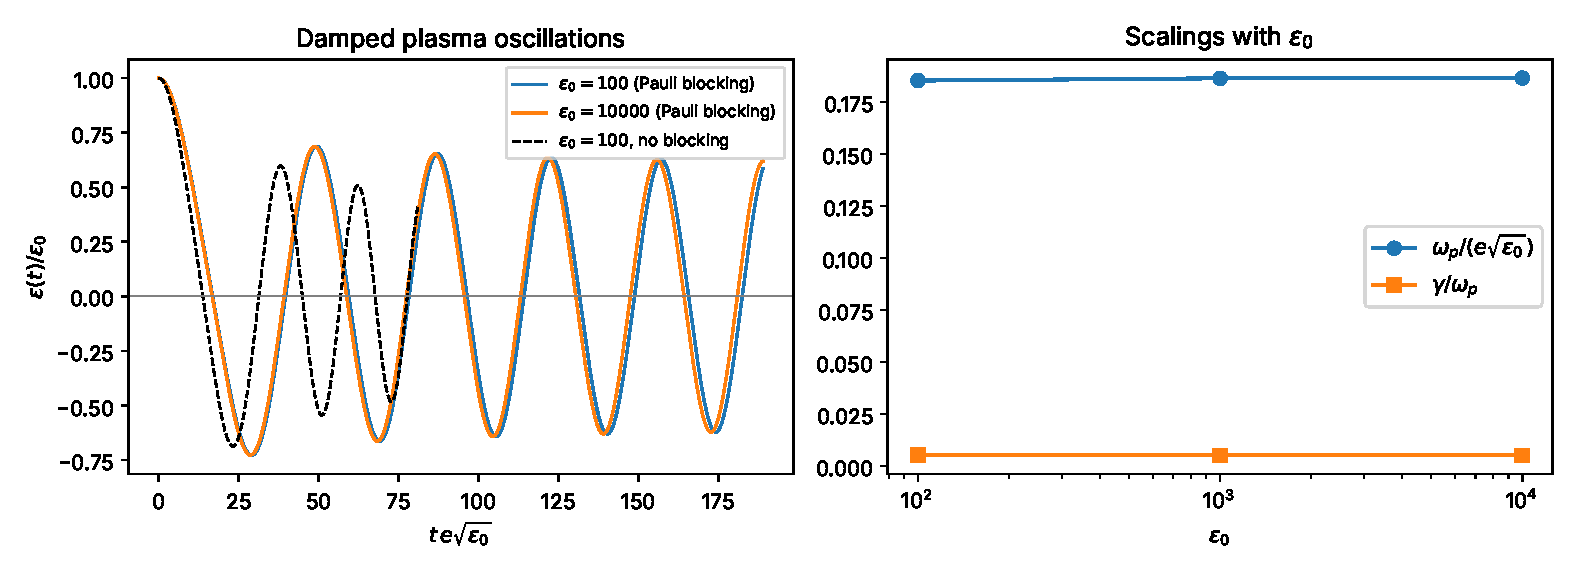
\includegraphics[width=0.92\textwidth]{fig_plasma_oscillations.pdf}
\caption{Left: electric field $\eps(t)/\eps_0$ in units of $1/(e\sqrt{\eps_0})$ for the Pauli-blocked Markov kinetic equation (solid) and without blocking (dashed), exhibiting the collapse of different $\eps_0$ onto one curve (scale invariance). Right: $\omega_p/(e\sqrt{\eps_0})$ and $\gamma/\omega_p$ as functions of $\eps_0$.}
\label{fig:plasma}
\end{figure*}

\subsection{Exact non-Markovian quantum kinetics}\label{sec:exact}
The Markov limit is removed by evolving, for every mode $(P,s{=}p_\perp^2)$ with kinetic momentum $p=P+\Phi(t)$, $\dot\Phi=x$ and $m_\perp^2=1+s$, the Bloch vector of the exact two-level Dirac problem $H=p\,\sigma_z+m_\perp\sigma_x$, with $f=(1-z)/2$, $u$ and $v$ the components of the Bloch vector along the adiabatic axes (Bloch--Bogoliubov form of the quantum Vlasov equation \cite{kluger1998,schmidt1998}):
\begin{align}
\dot f&=\tfrac12\lambda\,u,\quad \dot u=\lambda(1-2f)-2\omega v,\quad \dot v=2\omega u,\label{eq:bloch}\\
\dot x&=-2e^2\sum W\Big[\frac p\omega f+\frac{m_\perp}{2\omega}u\Big],\quad \lambda=\frac{x\,m_\perp}{\omega^2},\label{eq:maxw}
\end{align}
with $\omega=\sqrt{p^2+m_\perp^2}$, $\rho_{\rm pl}=2\sum W\omega f$ and the parallel pressure $P_\parallel=\sum Wp\,[2(p/\omega)f+(m_\perp/\omega)u]$ (Hellmann--Feynman). There is no source term, no locally-constant-field approximation and no source width: phase coherence between successive crossings and Pauli blocking are contained exactly. SymPy derives Eq.~\eqref{eq:bloch} from $\dot{\bf n}=2{\bf h}\times{\bf n}$ together with the velocity and energy identifications (Q0), proves that $\frac{d}{dt}[(1-2f)^2+u^2+v^2]=0$ identically, so that the vacuum $(0,0,0)$ implies $0\le f\le1$ without any truncation at $\tfrac12$ (Q1), proves $\frac{d}{dt}(x^2/2e^2+\rho_{\rm pl})=0$ with the polarization current of Eq.~\eqref{eq:maxw} (Q2; omitting it leaves the residual $W x\,m_\perp u/\omega\neq0$, control C10), and the trace identity $\rho_{\rm pl}-P_\parallel-2P_\perp=\sum W m^2(2f-pu/m_\perp)/\omega$ (Q4).

\textbf{Normalization of the coupling.} The form $\dot f=\lambda u$, $\dot u=2\lambda(1-2f)-2\omega v$ (the coupling of Eq.~\eqref{eq:bloch} doubled) is not excluded by the algebraic gates: it also conserves purity and energy (with a correspondingly doubled polarization current), so these gates cannot discriminate it, but it fails the Landau--Zener test: for $eE=10$, $m_\perp=1$ it gives $f_\infty=0.2942$ instead of $e^{-\pi m_\perp^2/eE}=0.7304$ (control C11). The coefficient of Eq.~\eqref{eq:bloch} is the one derived from the Dirac equation (Q0) and reproduces $f_\infty=e^{-\pi m_\perp^2/eE}$ to $\ensuremath{4.1\times10^{-7}}$ or better in all $8$ test cases (Q3; the C kernel gives $\ensuremath{2.1\times10^{-6}}$, Q3b), with $f_\infty$ up to $0.969$, above the Markov ceiling $\tfrac12$ for $\eps>\pi/\ln2=4.5324$ (Q3a).

\textbf{Numerics.} A fixed-step RK4 scheme in C/OpenMP (time step $0.2/\omega_{\max}$, $P$-spacing $0.04\sqrt{\eps_0}$, 30 Gauss--Legendre nodes in $p_\perp^2$) integrates $39450$ modes at $\eps_0=100$. The discrete system conserves $x^2/2e^2+\rho_{\rm pl}$ exactly, and the integrator preserves it to $\ensuremath{6.2\times10^{-12}}$ over at least five oscillations for $\eps_0\ge10$ (Q2b). Halving $\Delta P$ or $\Delta t$, doubling the transverse nodes or widening the $P$ range changes $\tau_0$ by $\le\ensuremath{1.7\times10^{-8}}$ and the first four half-periods by $\le\ensuremath{3.4\times10^{-3}}$ (K6); a narrow $P$ range is detected by the coverage gate (C12). The initial state is the zeroth-order adiabatic vacuum at $t=0$, as in the Markov model; replacing it with the first-order superadiabatic vacuum changes the first half-periods by $\ensuremath{1.5\times10^{-2}}$ (K8).

\textbf{Results} (Table~\ref{tab:exact}, Fig.~\ref{fig:exact}). The exact system is not capped at $\tfrac12$: $f_{\max}=0.999996$ at $\eps_0=100$ and $\ge0.99997$ for every $\eps_0\ge10$ (Q1c), against $0.5000$ for the blocked Markov model; even at $\eps_0=4<\pi/\ln2$ interference between successive crossings reaches $f_{\max}=0.9990$. For a single crossing the blocked Markov rule undershoots by the fraction $0.536$ at $f_0=0.9$ (limit $0.568$ for $f_0\to1$). The first zero of the field occurs earlier than in the Markov model: $\tau_0e\sqrt{\eps_0}=13.44$ at $\eps_0=10^3$ against $16.67$, a ratio $0.806$ ($0.851$ at $\eps_0=10$, $0.899$ at $\eps_0=4$). The exact value is within $0.8$ per cent of the constant $\kappa=13.54$ of the unblocked source of Sec.~\ref{sec:kinetic}, so the lengthening attributed above to Pauli blocking is an artefact of the ceiling at $\tfrac12$. The plasma frequency (mean of the last three half-periods) scales as $\omega_p\propto\eps_0^{0.505}$ with $\omega_p/(e\sqrt{\eps_0})=0.1944$ for $\eps_0=10^3$, i.e.\ $4.3$ per cent above the Markov value $0.1864$ (K7). The amplitude decays slowly and non-exponentially (it falls from $0.78$ to $0.67$ of $E_0$ in six half-cycles), and the log-linear fit gives $\gamma/\omega_p=0.0048$ against $0.0052$; with ten amplitudes this number is a rough descriptor and the difference is not significant. \emph{Equation of state.} The total parallel $w_{\rm tot}=(P_\parallel-E^2/2)/(\rho_{\rm pl}+E^2/2)$ starts at $-1$ (pure field) and first reaches zero at $t\,e\sqrt{\eps_0}=6.23$ ($6.57$ at $\eps_0=30$), before the first field zero at $13.4$. The pairs themselves have $w_\parallel^{\rm pl}=P_\parallel/\rho_{\rm pl}>\tfrac13$ from the first instant ($t\,e\sqrt{\eps_0}\simeq0.020$) and its average over the last period is $0.988$ (at most $1.054$ instantaneously, the excess over unity being the coherent term): it tends to the collinear value $1$, not to the isotropic $\tfrac13$, because the pairs are created with $p_\perp^2\sim\eps/\pi\ll p_\parallel^2$ and the homogeneous model has no collisions or transverse spreading that could isotropize them. \emph{Controls and sensitivity.} Without the polarization current the energy drifts by $\ensuremath{4.1\times10^{-2}}$ (C13); with the doubled coupling (and a consistent doubled current) energy is conserved but $\tau_0e\sqrt{\eps_0}$ changes to $15.18$ (C14), so only Landau--Zener fixes the coefficient. The initial state is the zeroth-order adiabatic vacuum; the first-order superadiabatic vacuum changes $\tau_0$ by $0.015$ of its value (K8).

\begin{table*}[t]
\caption{Exact (Bloch--Bogoliubov) versus Markov kinetics at the same $\eps_0$: maximum occupation, first zero $\tau_0e\sqrt{\eps_0}$, plasma frequency $\omega_p/(e\sqrt{\eps_0})$ (mean of the last three half-periods), $\gamma/\omega_p$ (log-linear fit of the half-cycle amplitudes), and the time-averaged parallel equation of state of the pairs over the last period. For $\eps_0=4$ only four zero crossings were computed.}
\label{tab:exact}
\begin{ruledtabular}
\begin{tabular}{rccccccccc}
$\eps_0$ & $f_{\max}^{\rm ex}$ & $f_{\max}^{\rm M}$ & $\tau_0^{\rm ex}$ & $\tau_0^{\rm M}$ & $\omega_p^{\rm ex}$ & $\omega_p^{\rm M}$ & $\gamma/\omega_p^{\rm ex}$ & $\gamma/\omega_p^{\rm M}$ & $\langle w_\parallel^{\rm pl}\rangle$\\\hline
4 & 0.99902 & 0.47109 & 21.29 & 23.69 & 0.1236 & 0.1169 & 0.0140 & 0.0167 & 0.991\\
10 & 1.00000 & 0.50000 & 16.17 & 19.01 & 0.1790 & 0.1740 & 0.0047 & 0.0057 & 0.988\\
30 & 1.00000 & 0.50000 & 14.28 & 17.38 & 0.1907 & 0.1824 & 0.0044 & 0.0053 & 0.988\\
100 & 1.00000 & 0.50000 & 13.67 & 16.86 & 0.1947 & 0.1853 & 0.0047 & 0.0052 & 0.988\\
300 & 0.99999 & 0.50000 & 13.50 & 16.72 & 0.1945 & 0.1861 & 0.0045 & 0.0052 & 0.988\\
1000 & 0.99997 & 0.50000 & 13.44 & 16.67 & 0.1944 & 0.1864 & 0.0048 & 0.0052 & 0.988\\
\end{tabular}
\end{ruledtabular}
\end{table*}

\begin{figure*}[t]
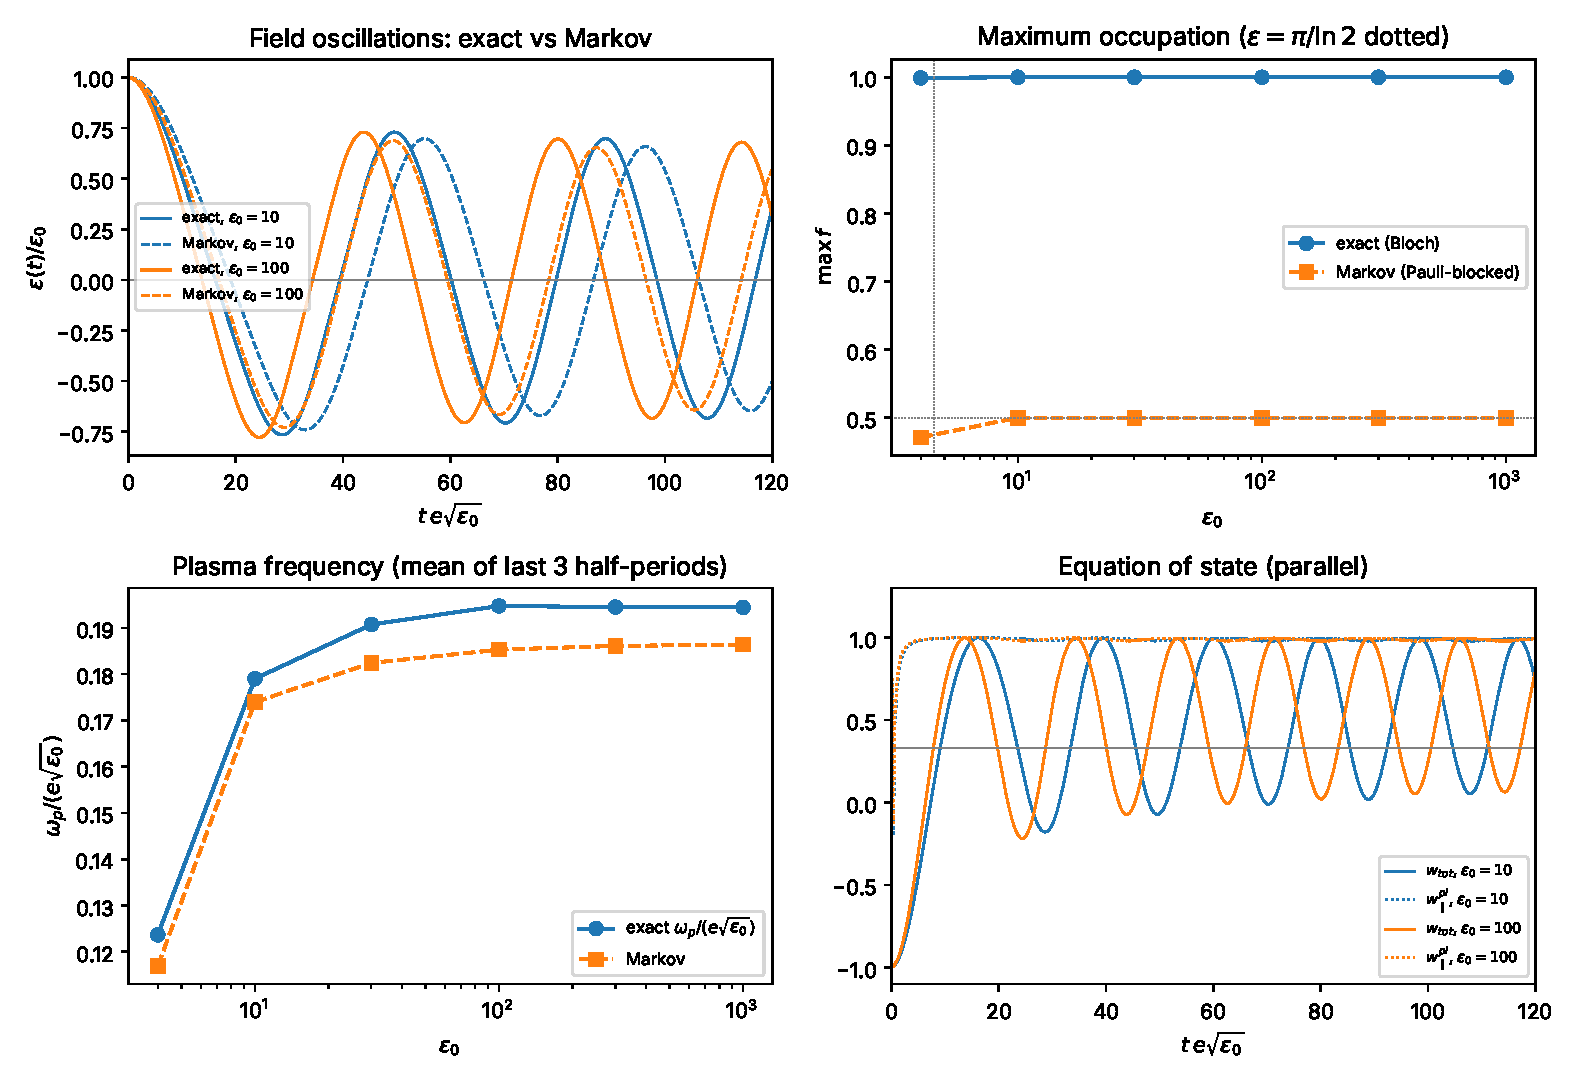
\includegraphics[width=0.92\textwidth]{fig_markov_vs_exact.pdf}
\caption{Exact non-Markovian quantum Vlasov (solid) versus the Pauli-blocked Markov model (dashed). Top left: field oscillations at $\eps_0=10$ and $100$. Top right: maximum occupation $f$; the exact system exceeds the Markov ceiling $\tfrac12$ above $\eps=\pi/\ln2$. Bottom left: plasma frequency. Bottom right: parallel equation of state $w_{\rm tot}=(P_\parallel-E^2/2)/(\rho_{\rm pl}+E^2/2)$ (solid) and $w_\parallel^{\rm pl}=P_\parallel/\rho_{\rm pl}$ (dotted).}
\label{fig:exact}
\end{figure*}

\section{Scales and phase map}\label{sec:phase}
For $N$ electrons of charge $Ne$ confined in radius $r_0$ (lengths in $\lC$): the field reaches $\eps=1$ at $r_\eps=\sqrt{N\alpha}$; the Reissner--Nordstr\"om radius is $r_Q=N\sqrt\alpha/\MPl$; the Coulomb density equals $\MPl^4$ at $r_P$ (with a floor of $10\,l_P$); and the trapping radius $r_s(N)$ solves $r=2G\,[N+\tfrac34(9\pi/4)^{1/3}N^{4/3}/r]$ (rest mass plus ultra-relativistic Fermi energy, gate P4). Because of the cancellation of Sec.~\ref{sec:trap}, $r_s$ is independent of the charge. The ratio of the electromagnetic to the gravitational force of the electron is $z^2=\alpha\MPl^2=\ensuremath{4.17\times10^{42}}$.

\textbf{Time scales.} With $E_0=Q/4\pi r_0^2$, $\eps_0=N\alpha/r_0^2$ and the result of Sec.~\ref{sec:kinetic}, $\tau_{\rm dis}=\kappa\,r_0/(\alpha\sqrt{4\pi N})$, equal to the light-crossing time at $N^*=\kappa^2/(4\pi\alpha^2)=\ensuremath{2.74\times10^{5}}$. For the free fall of a dust ball of mass $Nm_e$, $\tau_{\rm ff}=\tfrac\pi2\sqrt{r_0^3/2GM}$ (symbolic, P8). Both times scale as $N^{-1/2}$, so
\begin{equation}
\frac{\tau_{\rm dis}}{\tau_{\rm ff}}=\sqrt{\frac{r_0^*}{r_0}},\qquad r_0^*=\frac{2\kappa^2}{\pi^3\alpha^2\MPl^2}=\ensuremath{9.29\times10^{-18}}\,l_P ,
\label{eq:ratio}
\end{equation}
independent of $N$ (gate P9). We stress that this closed form is the product of two power laws and of the electron's $z^2$; it only expresses that discharge is faster than free fall for every $r_0>l_P$ (since $r_0^*\ll l_P$ the value of $r_0^*$ itself lies outside the validity of either model). On the trapping boundary with the Fermi energy included, the discharge wins only for $N\gtrsim\ensuremath{1.11\times10^{5}}$ \emph{if the charge carriers stay in place}; Sec.~\ref{sec:shell} shows that the Coulomb push, not free fall, sets the relevant clock, and that it is lost at every $N$ in the shell model.

\textbf{Phase map} (Fig.~\ref{fig:phase}). Four regions: static EFT ($\eps<1$); Schwinger discharge ($r_P<r_0<r_\eps$ and untrapped); trapping ($r_0\le r_s$); and trans-Planckian. The trapped region always lies at $\eps\gg1$ and above the Planck floor for $N\gtrsim15$; a classical horizon enters the static-EFT region only for $N\gtrsim\alpha\MPl^4/4=\ensuremath{5.94\times10^{86}}$. The Coulomb density at $r_Q$ is $\rho/\MPl^4=1/(8\pi\alpha N^2)$ (P6), sub-Planckian for $N\ge$2.3. The ``trapping'' region $r_0\le r_s$ is the shell criterion $2GM_n\ge r_0$ (matter surface with no interior field energy); Sec.~\ref{sec:dyn1d} shows that for $N>N_A\simeq\ensuremath{4.6\times10^{4}}$ this curve lies inside the region $r_0\le0.6\,r_Q$ in which the initial data of a uniformly charged ball already contain an apparent horizon. Table~\ref{tab:scales} lists the scales. The electrons in region (ii) are not bound (the Coulomb energy exceeds the Fermi energy for $N\gtrsim\ensuremath{6.0\times10^{3}}$); $r_s$ is a condition on initial data, not a formation scenario.

\begin{figure*}[t]
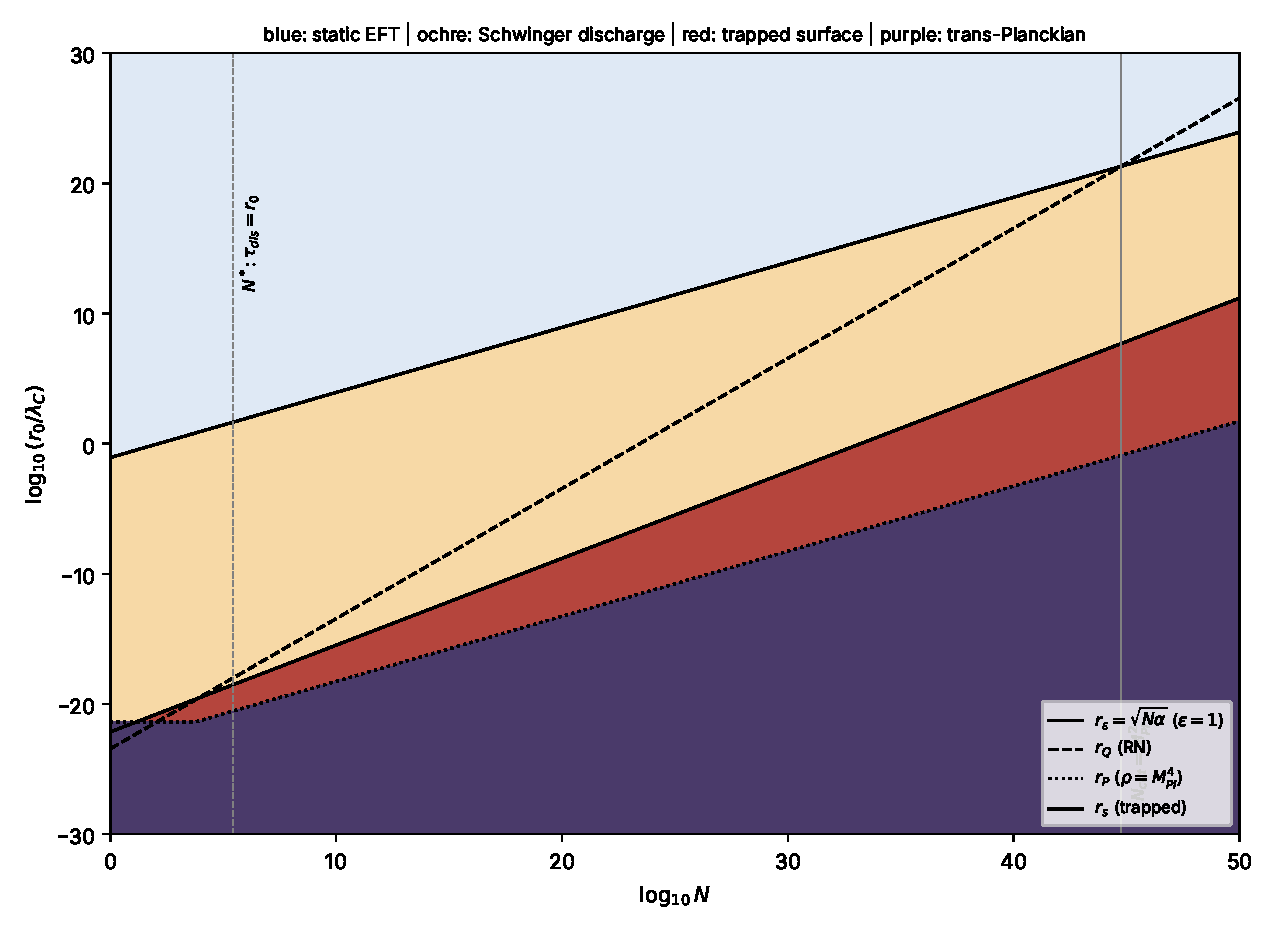
\includegraphics[width=0.78\textwidth]{phase_diagram.pdf}
\caption{Phase map in the $(N,r_0)$ plane. Solid lines: $r_\eps=\sqrt{N\alpha}$ and $r_s(N)$; dashed: $r_Q$; dotted: Planck-density radius. Vertical lines mark $N_{\rm crit}=\MPl^2/m_e^2$ and $N^*$ ($\tau_{\rm dis}=r_0$).}
\label{fig:phase}
\end{figure*}

\begin{table*}[t]
\caption{Characteristic radii (in $\lC$) and ratios for selected $N$ (computed in \texttt{06\_phase\_diagram.py}).}
\label{tab:scales}
\begin{ruledtabular}
\begin{tabular}{rccccc}
$N$ & $r_\eps$ & $r_Q$ & $r_s$ & $\eps(r_s)$ & $\tau_{\rm dis}/r_0$\\\hline
$1.00\times10^{0}$ & $8.54\times10^{-2}$ & $3.58\times10^{-24}$ & $7.10\times10^{-23}$ & $1.45\times10^{42}$ & $5.23\times10^{2}$\\
$1.00\times10^{3}$ & $2.70\times10^{0}$ & $3.58\times10^{-21}$ & $7.10\times10^{-21}$ & $1.45\times10^{41}$ & $1.66\times10^{1}$\\
$1.00\times10^{6}$ & $8.54\times10^{1}$ & $3.58\times10^{-18}$ & $7.10\times10^{-19}$ & $1.45\times10^{40}$ & $5.23\times10^{-1}$\\
$1.00\times10^{12}$ & $8.54\times10^{4}$ & $3.58\times10^{-12}$ & $7.10\times10^{-15}$ & $1.45\times10^{38}$ & $5.23\times10^{-4}$\\
$1.00\times10^{20}$ & $8.54\times10^{8}$ & $3.58\times10^{-4}$ & $1.53\times10^{-9}$ & $3.12\times10^{35}$ & $5.23\times10^{-8}$\\
$1.00\times10^{30}$ & $8.54\times10^{13}$ & $3.58\times10^{6}$ & $7.10\times10^{-3}$ & $1.45\times10^{32}$ & $5.23\times10^{-13}$\\
$5.71\times10^{44}$ & $2.04\times10^{21}$ & $2.04\times10^{21}$ & $4.89\times10^{7}$ & $1.74\times10^{27}$ & $2.19\times10^{-20}$\\
$1.00\times10^{48}$ & $8.54\times10^{22}$ & $3.58\times10^{24}$ & $7.10\times10^{9}$ & $1.45\times10^{26}$ & $5.23\times10^{-22}$\\
$1.00\times10^{60}$ & $8.54\times10^{28}$ & $3.58\times10^{36}$ & $7.12\times10^{17}$ & $1.44\times10^{22}$ & $5.23\times10^{-28}$\\
\end{tabular}
\end{ruledtabular}
\end{table*}

\subsection{Spatially resolved discharge and trapping}\label{sec:dyn1d}
We evolve the system of Sec.~\ref{sec:dyn} on a radial grid in polar--areal gauge (script \texttt{06b\_dynamical\_trapping\_1d}; units $r_0=c=1$, $q=r_Q/r_0$, $s=\sqrt{N/N_*}$). The field of a uniformly charged ball, $\tilde\rho_{\rm EM}\propto q^2r^2$ ($r<1$) and $q^2/r^4$ ($r>1$), is converted locally with the clock $\dot s_c=\alpha\,\kappa s\sqrt{E/E_{\rm surf}}$ and the universal first-oscillation curve of the exact kinetics (Sec.~\ref{sec:exact}): the field decays as $E=E_{\rm geom}\,g(s_c)$ until its first zero, the energy removed is shared equally between an outgoing and an ingoing null stream (zero net momentum; the collinear plasma of Sec.~\ref{sec:exact} has $w_\parallel\simeq1$), and the metric follows from the constraints at every step. At the surface the discharge time is $r_0/s$ (so $s=1$ is $N=N_*$). The held mass $M_n$ enters as a static test mass. The flat limit with instantaneous discharge has a closed form, including the passage of ingoing rays through the centre: the solver reproduces $E_{\rm out}$ and $E_{\rm in}$ to $\ensuremath{1.3\times10^{-5}}$ and $\ensuremath{1.7\times10^{-6}}$ with observed order $2.00$ (N1; omitting the centre reflection gives an error of 3\%, control C\_N1). In the full theory the balance $m(r_0,t)-m(r_0,0)=\int(F_{\rm in}-F_{\rm out})dt$ of Eq.~\eqref{eq:msdyn} holds to $\ensuremath{1.0\times10^{-3}}$ relative ($\ensuremath{2.4\times10^{-5}}$ absolute) in 10 cases with $q$ up to 1.3 (N2); a plasma that receives $1.2\times$ what the field loses breaks it by $\ensuremath{4.0\times10^{-2}}$ (C\_N2). Grid convergence with $\Delta r$, $\Delta r/2$, $\Delta r/4$ is \ensuremath{5.5\times10^{-4}} at most (N3).

\textbf{How much mass-energy leaves, and how much arrives.} Take weak gravity ($q=0.2$) and instantaneous discharge, evaluated at $t=r_0/c$ (perfectly radial streams form a central caustic after that time; beyond it, up to the free-fall time $\tfrac\pi2r_0$ of the trapping boundary, a reflecting core of radius $r_{\rm core}=0.1\,r_0$ stands in for the angular momentum of the rays, $\theta_\perp\simeq\sqrt{1-w_\parallel}\simeq0.11$ from Sec.~\ref{sec:exact}; it conserves energy exactly, $|\Delta m-\!\int\!F|\le\ensuremath{2.4\times10^{-5}}$, changes $\Delta C$ by 0.049 for $r_{\rm core}=0.05\to0.2$ at $q=0.5$ and by $\ensuremath{3.4\times10^{-8}}$ at $q=1$, N10). A neutral matter element released from rest follows the radial geodesic of the evolving metric; in a point-mass test its proper fall time agrees with the exact cycloid to $\ensuremath{3.5\times10^{-5}}$ (N9), which validates $\alpha$, $a$, $\phi_r$ and $\lambda_t$ used for the dynamics. The interior channel (field energy inside the ball converted into plasma that crosses $r_0$ outwards) removes $\Delta C=\ensuremath{-0.0997}\,q^2$ from $C=2GM_{\rm MS}(r_0)/r_0$, i.e.\ a fraction $0.497$ of the interior field energy ($0.422$ for $s=1$) and $0.083$ of the total field energy $U_C$. The exterior channel (field energy outside the ball converted in place, whose ingoing half enters $r_0$) adds $0.2481\,q^2$, $2.49$ times larger, so the net effect is a \emph{gain}, $\Delta C=+0.1493\,q^2$: the quasilocal mass at the surface is increased, not decreased, by the discharge. The net gain depends on the discharge speed as $\Delta C\simeq q^2F_\infty s^p/(s^p+s_h^p)$ with $F_\infty=0.1493$, $p=1.61$, $s_h=1.62$ (N4, N8): it is the instantaneous-discharge value for $N\gg N_*$ and falls as $s^{p}$ for $N\ll N_*$, where the plasma escapes ballistically before the field is converted ($0.0065\,q^2$ at $s=0.3$). Gravity suppresses the inflow: at $q=1$, $\Delta C/q^2=0.096$ (instantaneous) and at $q=1.5$ it is $0.0004$, and a held mass $C_n=0\to0.6$ lowers $\Delta C$ at $q=1$, $s=3$ from $0.0626$ to $0.0011$, because the coordinate speed $v=\alpha/a$ vanishes as $\theta_+\to0$ (N5).

\textbf{Displacement of the trapping threshold.} Just below the static horizon threshold of P12, at $C_n=C_n^{\rm AH}(q)-0.05$ with $C_n^{\rm AH}=1-q^2/5$ for $q<1$ and $2q-\tfrac65q^2$ for $q\ge1$, the maximum of the compactness profile grows by at most $\delta C_n=0.0033$ until $t=r_0/c$ and $0.0080$ until the free-fall time $\tfrac\pi2r_0$, over $q\in[0.3,1.5]$ and $s\in[0.1,\infty)$ ($0.0035$ at $s=1$); no case forms a new horizon, and the numerical initial compactness reproduces the closed form to $\ensuremath{4.3\times10^{-3}}$ (N6). Therefore the dynamics shifts the critical non-electromagnetic mass, $\Delta M_{\rm crit}/M_{\rm crit}$, by at most $0.0080$ ($0.8$\%) within the free-fall time, and in no regime does the escaping plasma delay trapping: the effect that dominates the retained mass is the \emph{static} interior field energy $q^2/5$, which the shell criterion of Sec.~\ref{sec:phase} omits. Figure~\ref{fig:dyntrap} shows the resulting curves in the $(N,r_0)$ plane: the horizon boundary $r_{\rm AH}(N)$ of the ball (P12 plus dynamics) lies above the shell curve $r_s(N)$ by a factor up to $1402$ for $N\le10^{14}$, the two cross at $N_A\simeq\ensuremath{4.62\times10^{4}}$ (where $r_s=0.6r_Q$), and the dynamic correction is $r^{\rm dyn}/r_{\rm AH}-1\le\ensuremath{1.1\times10^{-3}}$. For $N>N_A$ the curve $r_s(N)$ of the previous sections lies \emph{inside} the region where the initial data already contain an apparent horizon; there the race between discharge and free fall (Eq.~\eqref{eq:ratio}) is moot, because discharge cannot remove a trapped surface that already exists.

\begin{figure*}[t]
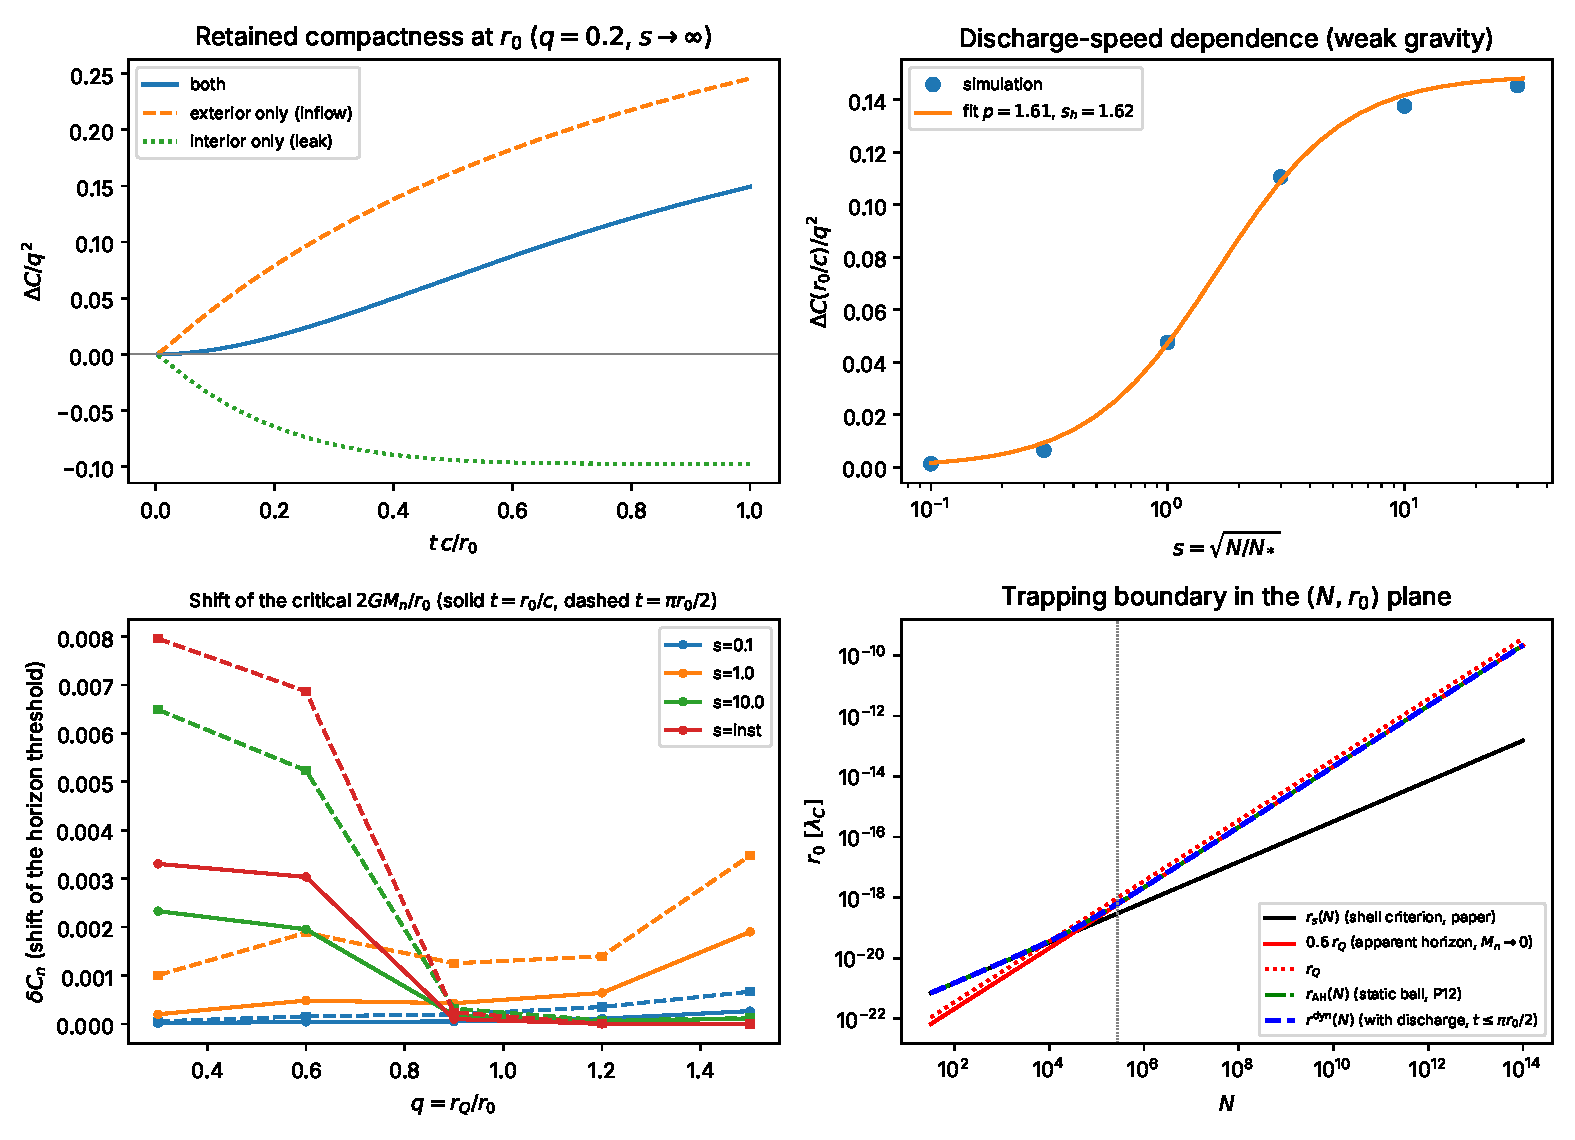
\includegraphics[width=0.92\textwidth]{fig_dynamic_trapping.pdf}
\caption{Spatially resolved discharge. Top left: retained compactness at $r_0$ for the interior (leak), exterior (inflow) and combined channels ($q=0.2$, instantaneous discharge). Top right: dependence on $s=\sqrt{N/N_*}$ and fit. Bottom left: shift $\delta C_n$ of the critical $2GM_n/r_0$ produced by the dynamics (solid: $t=r_0/c$; dashed: $t=\pi r_0/2$ with a reflecting core). Bottom right: boundaries in the $(N,r_0)$ plane: shell criterion $r_s$, $r_Q$ and $0.6\,r_Q$, apparent-horizon boundary of the static ball $r_{\rm AH}$ and the corrected curve $r^{\rm dyn}$ (indistinguishable from $r_{\rm AH}$ at this scale).}
\label{fig:dyntrap}
\end{figure*}

\begin{figure}[t]
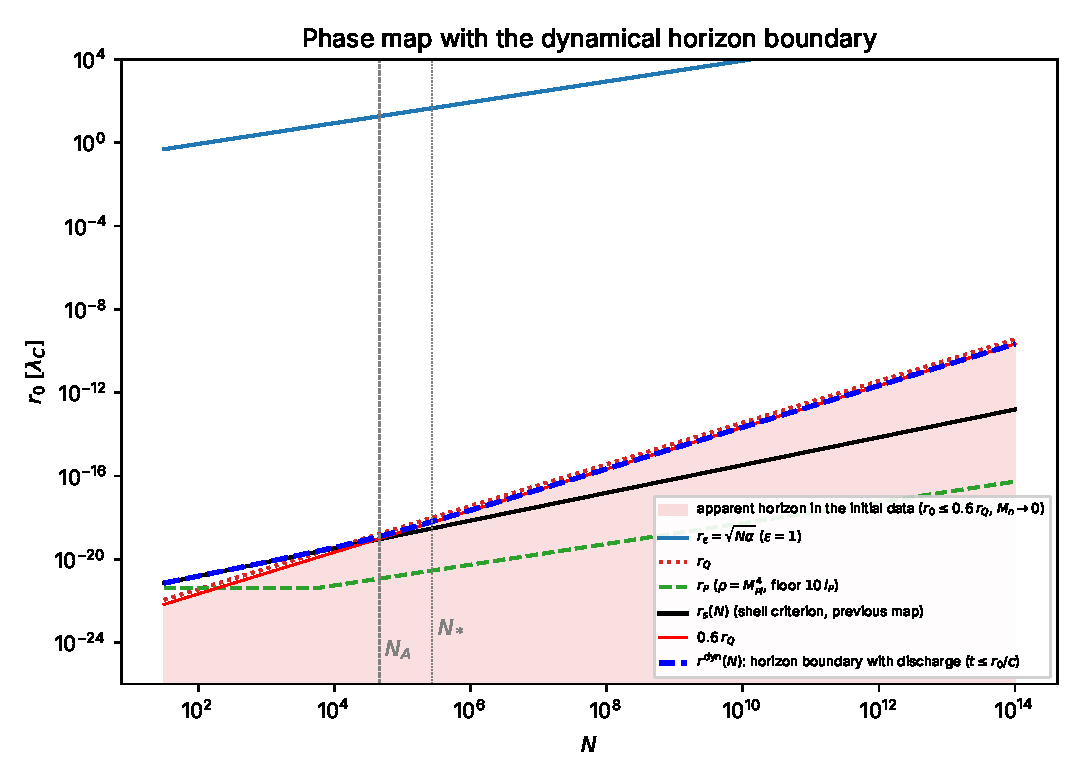
\includegraphics[width=\columnwidth]{phase_diagram_corrected.pdf}
\caption{Phase map of Fig.~\ref{fig:phase} with the horizon boundary of the charged ball: the shaded region has an apparent horizon in the initial data for arbitrarily small $M_n$; the curve $r^{\rm dyn}(N)$ includes the discharge up to $t=\pi r_0/2$ and coincides with $r_{\rm AH}$ to $10^{-3}$. For $N>N_A$ the shell curve $r_s$ lies inside the shaded region.}
\label{fig:phasecorr}
\end{figure}

\subsection{Self-consistent collapse of a charged shell: the race against the Coulomb push}\label{sec:shell}
The 1+1D solver holds the matter at $r_0$. To evolve the matter itself we use its exact thin-shell limit, which in Misner--Sharp variables is the Israel junction \cite{israel1966}: a shell of rest-mass compactness $C=2GM_n/r_0$ and charge $q=r_Q/r_0$, flat inside ($m_-=0$), with $E\equiv m_+$ the Misner--Sharp compactness just outside it, obeys
\begin{equation}
\Gamma_--\Gamma_+=\frac{C}{2R},\quad \Gamma_\pm^2=1-\frac{m_\pm}{R}+\dot R^2\;\Rightarrow\;\dot R^2=\Big(\frac C{4R}+\frac EC\Big)^2-1,\label{eq:israel}
\end{equation}
($R$ in units of $r_0$, dot = proper time). The exterior field energy $q^2g^2/R$ is the reservoir of the Coulomb work, $dE=q^2g^2\,dR/R^2$, where $g(s_c)$ is the screening of the field by the discharge (the universal curve of Sec.~\ref{sec:exact}, with the clock $\dot s_c=\kappa s/R$ at the shell). SymPy proves (P13) that, without discharge ($g=1$), a shell released from rest has $\dot R^2(1)=0$ and $d\dot R^2/dR|_1=2(q^2/C-C/4)$: it collapses \emph{if and only if} $q<C/2$ ($Q<\sqrt{4\pi G}\,M$) and otherwise expands to infinity, because its binding margin is only $C-E_0=C^2/4$; the initial data contain an apparent horizon for $q\ge2-C/2$. The integral $\dot R^2=F(R)$ is conserved by the numerical integration to $\ensuremath{1.7\times10^{-13}}$ and the neutral shell is trapped at $R=E_0$ with the Israel quadrature time (S1; omitting the Coulomb work, or mis-normalising the equation of motion, is detected, C\_S1).

With the discharge, the push before the screening completes gives $\Delta E=(q^4/C)\,I/(\kappa s)^2$ with $I=\int g^2\!\int g^2\,ds=19.756$, and the shell remains bound only if $\Delta E<C^2/4$:
\begin{equation}
s>s_c=\frac{2\sqrt I}{\kappa}\,\frac{q^2}{C^{3/2}}=0.657\,\frac{q^2}{C^{3/2}} .\label{eq:race}
\end{equation}
The simulation of the full shell dynamics gives the same law, $s_c\propto q^{2.012}C^{\ensuremath{-1.508}}$ with $A=0.6682$ (spread $\ensuremath{1.3\times10^{-2}}$, $\ensuremath{1.8\times10^{-2}}$ from Eq.~\eqref{eq:race}) over $C\in[0.03,0.3]$, $q\in[0.5,1.5]$ (S3). For $s>s_c$ the shell is trapped with a Misner--Sharp mass \emph{larger} than the neutral one, $\Delta E/E_0=\tfrac C4(s_c/s)^2$ ($\ensuremath{6.14\times10^{-3}}$, $\ensuremath{9.82\times10^{-4}}$, $\ensuremath{6.13\times10^{-5}}$ at $s/s_c=2,5,20$): in the self-consistent collapse the energy at the surface also increases, by at most $C/4$ of its value (S4).

The physical charge-to-mass ratio is fixed by constants: for rest mass $q/C=\tfrac12\sqrt\alpha M_{\rm Pl}=\ensuremath{1.02\times10^{21}}$, independent of $N$ and $r_0$ (this is the electron's $z^2$ in disguise). Eq.~\eqref{eq:race} then requires $s_c\simeq\ensuremath{2.1\times10^{31}}\sqrt q$, i.e.\ $N\gtrsim N_*s_c^2\simeq\ensuremath{1.3\times10^{68}}$ for $q\sim1$, against $N_{\rm crit}=M_{\rm Pl}^2=\ensuremath{5.7\times10^{44}}$. Over the whole admissible region of the $(N,r_0)$ plane ($C/2<q<2-C/2$ and $\eps_0\ge30$, for $N\le M_{\rm Pl}^2$) the ratio $s_c/s(N)$ is never below $2.33$ (reached at $N=\ensuremath{2.7\times10^{3}}$, where the Fermi energy dominates the mass), and equals $10^{0.5}$, $10^{3.4}$, $10^{8.4}$ and $10^{13.2}$ at $N=10^4,10^{10},10^{20},10^{40}$ (S5; Fig.~\ref{fig:shell}). In this decoupled estimate the discharge loses the race against the Coulomb unbinding of the charge carriers at every $N$; Sec.~\ref{sec:coupled} shows that the gravity of the converted plasma lowers the threshold substantially, so these orders of magnitude are an upper bound. What stands in any case is that the relevant competitor of the discharge is the Coulomb push, not free fall, so the comparison of Eq.~\eqref{eq:ratio} is not the right race.

\begin{figure*}[t]
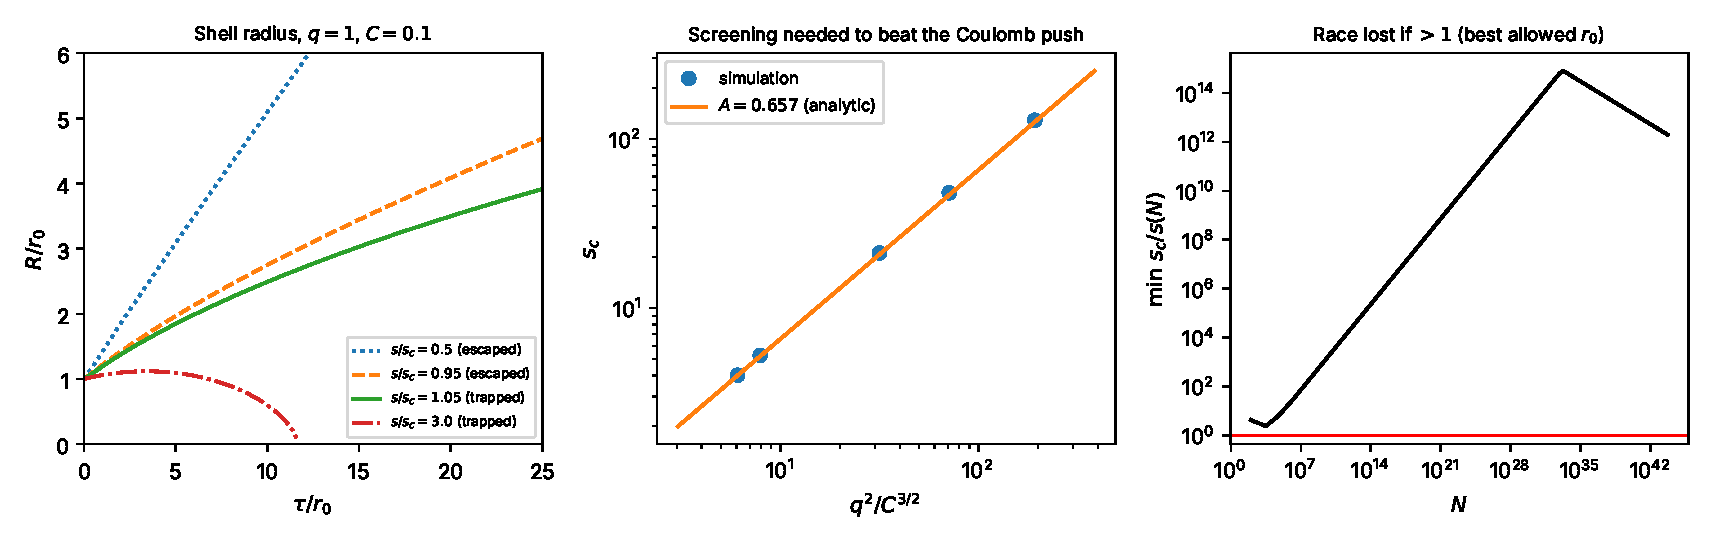
\includegraphics[width=0.95\textwidth]{fig_shell_race.pdf}
\caption{Charged-shell collapse (Israel junction with discharge screening). Left: shell radius for screening speeds around the critical value $s_c$ ($q=1$, $C=0.1$). Centre: critical screening $s_c$ versus $q^2/C^{3/2}$ (points: simulation; line: analytic law, Eq.~\eqref{eq:race}). Right: best (minimum over the admissible $r_0$) ratio $s_c/s(N)$ with the physical $q/C$; the discharge wins only below the red line.}
\label{fig:shell}
\end{figure*}

\subsection{Fully coupled system: dynamical shell, plasma, field and discharge}\label{sec:coupled}
The shell is now matter of the polar--areal solver itself (script \texttt{dynshell}), with no test mass and no decoupling. Its energy $E_d=\tilde\mu\sqrt{1+w^2}/a$, radial momentum flux $P_d=E_dw^2/(1+w^2)$ and energy flux $E_d\dot R$ enter the Einstein constraints (mass jump $E_d$; lapse jump $\Delta\phi=\tfrac12a^2P_d/r$ from the radial stress of the moving shell; $\lambda_t$ from its flux); it moves on the radial geodesic of the metric without its own delta plus the proper Coulomb acceleration $q^2g^2/(CR^2)$; the exterior field $q^2g(s_c)^2/r^4$ ($r>R(t)$) is converted locally into the two null streams, which cross the shell freely and gravitate on it; and cells left behind by a contracting shell inherit the screening of their outer neighbour (Gauss continuity). Validation: in vacuum the proper time to $R=0.7$ differs from the exact Israel quadrature by $0.032$ ($C=0.3$) and $0.013$ ($C=0.1$), i.e.\ it is $O(C)$ (self-gravity of the smeared shell), with grid variation $\ensuremath{7.4\times10^{-4}}$; the shell energy is constant to $\ensuremath{7.4\times10^{-4}}$; a doubled self-gravity is detected ($\ensuremath{-0.27}$) (K1). The total energy of field, plasma and shell obeys $\Delta m(R_{\max})=-\!\int\!F$ to $\ensuremath{5.2\times10^{-4}}$ over a full collapse ($m_0=1.035$); without discharge the shell with $q=1\gg C/2$ explodes, and removing the Coulomb force breaks the balance by $\ensuremath{7.2\times10^{-1}}$ (K2).

\textbf{Result: the plasma binds the shell.} The escape threshold of the coupled system, $s_c^{\rm cpl}$, is lower than the decoupled law of Eq.~\eqref{eq:race} (K3): $5.00$ against $20.76$ at $(q,C)=(1,0.1)$, $3.08$ against $5.19$ at $(0.5,0.1)$, $2.67$ against $46.72$ at $(1.5,0.1)$ and $1.53$ against $4.00$ at $(1,0.3)$, because the converted field energy ($\sim q^2$, larger than $C$) falls through the shell and attracts it. The $q^2$ dependence of the decoupled law is not present: $s_c^{\rm cpl}C$ stays within a factor $1.9$ ($0.27$--$0.50$) over $q\in[0.5,1.5]$, $C\in[0.1,0.3]$. A representative collapse ($q=1$, $C=0.1$, $s=21$) shows the answer to the question of mass loss in the coupled system: the Misner--Sharp compactness just outside the shell rises from $0.115$ to $0.973$ (the shell is at the threshold of trapping), the shell gains $0.013$ of its energy from the Coulomb push, and a fraction $0.40$ of the initial field energy leaves through the outer boundary as radiation; the radiated energy comes from the exterior field and does not reduce the mass at the shell. Extrapolating $s_c^{\rm cpl}\simeq\overline{s_cC}/C$ twenty decades to the physical $C=1/(q/C)$ (a purely numerical extrapolation, untested outside $C\in[0.1,0.3]$) gives $N\gtrsim\ensuremath{5.1\times10^{46}}$ against $N_{\rm crit}=\ensuremath{5.7\times10^{44}}$, i.e.\ much closer to the Planck number than the decoupled estimate $\ensuremath{1.3\times10^{68}}$, so the conclusion of Sec.~\ref{sec:shell} that the discharge loses the race by many orders of magnitude holds only for the decoupled estimate.

\section{What is known and what is specific to this work}\label{sec:attrib}
\begin{table*}[t]
\caption{Attribution of the results. ``Known'' means that the mathematical structure was published before; ``here'' lists what the pipeline adds.}
\label{tab:attrib}
\begin{tabular}{p{4.2cm}p{5.2cm}p{7.2cm}}\toprule
Result & Prior work & Contribution of this work\\\midrule
Coulomb energy cancels in trapping & Misner--Sharp mass with charge, thin-shell energy equation, charged Penrose inequality \cite{misner1964,hayward1994,boulware1973,malec1994,khuri2017} & Derivation inside a CAS under explicit hypotheses (time-symmetric data, $\rho\ge0$, no exterior charge); one-loop-exact $U_C(R)$\\
Plasma oscillations, Markov source, $\omega_p\propto e\sqrt{eE}$ & \cite{kluger1991,kluger1992,kluger1998,schmidt1998,ruffini2010,gelis2016} & Exact energy identity with $(1-2f)$ in $j_{\rm pol}$, $f\le\tfrac12$, constants $\omega_p$, $\gamma$ for this source; convergence and negative controls\\
Bloch--Bogoliubov quantum Vlasov with Maxwell back-reaction & \cite{kluger1998,schmidt1998,prakapenia2023} & Same equations (a rediscovery); here: symbolic Dirac$\to$Bloch derivation, a Landau--Zener test that fixes the normalization of the coupling, a like-for-like Markov--exact comparison ($\tau_0$, $\omega_p$, $\gamma$, $f_{\max}$) and the parallel equation of state; not compared with published curves\\
Strong-field logarithm, Landau scale & \cite{ritus1975,dunne2004} & Exact evaluation of the electric proper-time integral and the constant $K$\\
DEC violation & One-loop trace anomaly \cite{adler1977,collins1977} & Exact onset $\eps=$1.88218 and identity $x^3(\mathcal L_1/x^2)'$\\
Charged thin-shell collapse, unbinding for $Q>\sqrt{4\pi G}M$ & \cite{israel1966,boulware1973,bekenstein1971} (standard) & The screening law $s_c=A\,q^2/C^{3/2}$ for a discharging shell, derived analytically and verified by simulation, and its evaluation at the physical $q/C$; the closure of the discharge is an ansatz\\
Dynamical Misner--Sharp equations, quasilocal flux balance, radial null-dust transport in polar--areal gauge & \cite{misner1964,hayward1994} (standard) & Derivation in a CAS for the general $\phi(t,r),\lambda(t,r)$ metric with a Maxwell field and an exchange term, negative control for the transfer law; the conclusion that field$\to$plasma conversion inside $R$ conserves $M_{\rm MS}$ and only the surface flux counts is classical\\
Channel decomposition (leak from inside, inflow from outside) and its dependence on $q$ and $N/N_*$ & none found; radiation collapse of null shells is classical & Quantitative numbers for this specific discharge closure; not a prediction (closure ansatz, test-mass matter, radial beams)\\
Discharge of charged black holes, $N_{\rm crit}$ & Gibbons \cite{gibbons1975} & Reformulation of the scale in the $(N,r_0)$ plane\\
EH black holes (quartic) & \cite{yajima2001,ruffini2013} & Quantitative comparison with the exact one-loop interior in the coupled system, with explicit limits of validity\\
$\tau_{\rm dis}/\tau_{\rm ff}=(r_0^*/r_0)^{1/2}$, phase map & Elementary combination of known scalings & Closed forms with $\kappa$, verified symbolically; organization in one plane\\\bottomrule
\end{tabular}
\end{table*}

\section{Regimes where the model is not controlled}\label{sec:limits}
(1) \emph{Higher loops.} All strong-field statements are one-loop; Ritus--Narozhny scaling may invalidate them for $\eps\gtrsim10^3$--$10^6$. The sweep of the kinetic model reaches $\eps_0=10^{10}$, 6.8 orders above that threshold. (2) \emph{Derivative expansion and curvature.} The profiles of Sec.~\ref{sec:static} descend to $r\sim10^{-18}\lC$; the curvature couplings of the one-loop action \cite{drummond1980} are of relative order $\alpha(\lC/L)^2$ and are neglected, and the local-field Lagrangian is not controlled there. (3) \emph{Imaginary part.} For $\eps>1$ the vacuum-decay rate is $O(1)$ and the real part alone is not a stable effective action. (4) \emph{Kinetics.} The exact Bloch system of Sec.~\ref{sec:exact} has no LCFA and no $f\le\tfrac12$ cap, but it is homogeneous, has no collisions or spatial transport (the pairs do not isotropize: $\langle w_\parallel\rangle\simeq1$), starts from the zeroth-order adiabatic vacuum (a \ensuremath{1.5\times10^{-2}} effect on the half-periods), uses a finite $(P,p_\perp)$ quadrature (converged to \ensuremath{3.4\times10^{-3}}), and only reaches $\eps_0=10^3$; the Markov constants of Sec.~\ref{sec:kinetic} are model-specific, and the first-zero scale $\kappa$ of the cohort model (LCFA, Markov, $t_{\rm form}/\tau_0\simeq e/\kappa=0.022$) agrees with the exact kinetics only to the 0.8 per cent quoted in Sec.~\ref{sec:exact}. (5) \emph{Dynamics of trapping.} The dynamical Misner--Sharp balance is proven (Sec.~\ref{sec:dyn}); the 1+1D plasma solver with a static ball is validated but treats the matter as a test mass (constraint violation 0.17--0.31 of $\Delta C$); the fully coupled shell--plasma--field system of Sec.~\ref{sec:coupled} removes that approximation but has its own limits: the shell is a single smeared layer with $O(C)$ self-gravity error, the screening $g(s_c)$ is the local closure of the discharge (a permanent neutralization after the first zero, Gauss's law imposed only through the inheritance of the screening), the plasma is radial null streams with a reflecting core $r_{\rm core}=0.1r_0$ in place of angular momentum, the charged ball has no radial structure and the interior of the shell carries no field; collisions, transverse spreading, the many-body Coulomb explosion and the polar--areal gauge after the appearance of an apparent horizon are not treated, and the thresholds were computed only for $C\in[0.1,0.3]$, $q\in[0.5,1.5]$. (6) \emph{Landau and Planck.} The Landau pole and the Planck density are never crossed in any calculation; the Planck floor defines region (iii) and no statement is made there.

\section{Conclusions}\label{sec:concl}
Beyond the point where the quartic static EEH description fails, the exact one-loop static field does not saturate and does not censor the horizon; the electrostatic energy \emph{outside} the surface plays no role in the trapping of that surface, which for a shell requires non-electromagnetic mass, $GM_n\ge R/2$ (the interior field energy of a ball does gravitate, Sec.~\ref{sec:dyn}); and pair discharge converts the field into plasma on the time $\tau_{\rm dis}=\kappa/(e\sqrt{eE_0})$ while conserving energy-momentum, so it cannot remove mass or undo a trapped surface. In the exact homogeneous kinetics the resulting collinear pair plasma oscillates for many periods with $\omega_p\simeq0.194\,e\sqrt{eE_0}$ (the Pauli-blocked Markov model gave 0.186), reaches occupations up to unity, and has $\langle w_\parallel\rangle\simeq1$. What discharge does remove is the net charge whose repulsion exceeds gravity by $z^2\sim10^{42}$, and it does so faster than free fall, but not faster than the Coulomb push on the charge carriers (Sec.~\ref{sec:shell}). These conclusions are consistent with the classical picture of Misner--Sharp, Boulware and Gibbons; the added value of this work is a verified quantitative map of where each description holds, together with an open, reproducible pipeline. Collisional isotropization, a comparison with published non-Markovian curves and the evolution of the matter and of the plasma beyond the first light-crossing time (central caustic, formation of the horizon) remain open. The matter evolved as a charged shell is unbound by its own Coulomb push unless the screening exceeds a threshold that the gravity of the converted plasma lowers by a factor 0.24 with respect to the decoupled law ($s_c=0.66\,q^2/C^{3/2}$); whether the discharge reaches it at the physical $q/C$ depends on a twenty-decade extrapolation of this coupled threshold. For the spatial and gravitational gap, the complete Misner--Sharp balance with $K_{ij}\neq0$ is derived, the discharge of a charged ball is simulated, and the result is that the dynamics moves the horizon threshold by less than 0.8 per cent up to the prescribed free-fall time while the static interior field energy, absent from the shell criterion, relocates the threshold to $r_0\simeq0.6\,r_Q$ for large $N$.

\begin{acknowledgments}
The symbolic derivations, code and first draft of the text were produced with an AI assistant (Claude, Anthropic) operating the open pipeline described in Appendix~\ref{app:pipeline}; the author is responsible for the content. Bibliographic details marked in \texttt{references.bib} must be verified against the original publications before submission.
\end{acknowledgments}

\appendix
\section{Verification pipeline and reproducibility}\label{app:pipeline}
The repository (\url{https://github.com/lopezalmeidaalvaro/experimento}) contains numbered scripts executed by \texttt{run\_all.sh}, which stops at the first failing gate. Symbolic gates assert $\mathrm{simplify}(\mathrm{LHS}-\mathrm{RHS})=0$; numerical gates include convergence under refinement and an independent method; negative controls assert that altered signs, factors or conservation laws are detected. The totals are 123 gates, of which 25 are negative controls. Table~\ref{tab:gates} lists the gates by script.
\begin{table}[h]
\caption{Verification gates by script (symbolic, numerical and negative controls).}\label{tab:gates}
\begin{ruledtabular}
\begin{tabular}{p{3.0cm}rr}
Script & gates & neg.\ controls\\\hline
\texttt{04\_nonperturbative\_qed} & 22 & 3\\
\texttt{05\_dynamical\_backreaction} & 13 & 4\\
\texttt{05b\_plasma\_oscillations} & 12 & 4\\
\texttt{05c\_quantum\_vlasov\_exact} & 24 & 6\\
\texttt{06\_phase\_diagram} & 20 & 4\\
\texttt{06b\_dynamical\_trapping\_1d} & 32 & 4\\
01--03 (baseline) & \multicolumn{2}{r}{re-run at each build}\\
\end{tabular}
\end{ruledtabular}
\end{table}


\bibliography{references}
\end{document}
